\documentclass[17pt]{beamer}
\usepackage{tikz}
\usepackage{bera}

\beamertemplatenavigationsymbolsempty

\def\TCRESTblue{blue!70!green!75!white!60!black}
\def\TCRESTtextblue{blue!66!green!75!white!75!black}
\def\TCRESTred{red!70!black}
\def\TCRESTyellow{yellow!65!red!93!black}

\setbeamersize{text margin left=5.5mm}
\setbeamersize{text margin right=5.5mm}

\setbeamercolor{titlelike}{fg=\TCRESTtextblue}
\setbeamerfont{title}{size=\large}
\setbeamercolor{title page}{fg=\TCRESTtextblue}
\setbeamerfont{title page}{size=\large,series=\bf}
\setbeamerfont{author}{size=\small,series=\sf}
\setbeamercolor{author}{fg=black}
\setbeamercolor{section in toc}{fg=\TCRESTtextblue}
\setbeamerfont{section in toc}{series=\bf}

\setbeamercolor{author in head/foot}{fg=white}
\setbeamerfont{author in head/foot}{size=\fontsize{5.5}{5.5}}
\setbeamercolor{title in head/foot}{fg=white}
\setbeamerfont{title in head/foot}{size=\fontsize{5.5}{5.5}}
\setbeamercolor{page number in head/foot}{fg=white}
\setbeamerfont{page number in head/foot}{size=\fontsize{5.5}{5.5}}

\setbeamertemplate{title page}{%
  \vskip2.8cm
  \begin{center}
    \inserttitle
  \end{center}
  \vskip1cm
  \begin{center}
    \usebeamerfont{author}
    \usebeamercolor[fg]{author}
    \insertauthor
  \end{center}
}

\setbeamertemplate{background canvas}{%
  \begin{picture}(0,0)(4.8,1)
    \color{\TCRESTblue}%
    \linethickness{1.3mm}%
    \put(0,0){ \line(1,0){365} }
    \linethickness{5mm}%
    \put(0,-266){ \line(1,0){365} }
    \color{\TCRESTyellow}%
    \linethickness{.58mm}%
    \put(4.3,-2.7){ \line(1,0){365} }
    \put(4.3,-258){ \line(1,0){365} }
    \ifnum\theframenumber=1
    \put(15.9,-52.4) { 
\includegraphics[height=13.1mm]{logos/t-crest-logo} }
    \put(15.9,-66.7) { 
\includegraphics[width=120mm]{hline} }
    \else
    \put(308.4,-20.9){ 
\includegraphics[height=4.38mm]{logos/t-crest-logo} }
    \fi
  \end{picture}
}

\setbeamertemplate{frametitle}{%
  \vskip 2.5mm
  \usebeamerfont{title}\insertframetitle\\
  \vskip -4.4mm
  
\includegraphics[width=120mm]{hline}
}

\setbeamertemplate{footline}{%
  \leavevmode
  \hspace*{5mm}  
  \begin{beamercolorbox}[wd=34mm,ht=3.5mm,dp=1.5mm]{author in head/foot}%
    \raggedright\usebeamerfont{author in head/foot}\insertshortauthor
  \end{beamercolorbox}%
  \begin{beamercolorbox}[wd=50mm,ht=3.5mm,dp=1.5mm]{title in head/foot}%
    \centering\usebeamerfont{title in head/foot}\insertshorttitle
  \end{beamercolorbox}%
  \begin{beamercolorbox}[wd=33mm,ht=3.5mm,dp=1.5mm]{page number in head/foot}%
    \raggedleft\usebeamerfont{page number in head/foot}\insertframenumber
  \end{beamercolorbox}
}

\setbeamertemplate{itemize item}{\small{$\blacksquare$}}
\setbeamercolor{itemize item}{fg=\TCRESTred}
\setbeamertemplate{itemize subitem}{$\blacklozenge$}
\setbeamercolor{itemize subitem}{fg=\TCRESTtextblue}
\setbeamertemplate{itemize subsubitem}{$\bullet$}
\setbeamercolor{itemize subsubitem}{fg=\TCRESTred}

\setlength{\leftmargini}{1.5em}
\setlength{\leftmarginii}{1.1em}
\setlength{\leftmarginiii}{0.9em}

\author[Presenter, DTU]{Presenter\\Technical University of Denmark\\\href{mailto:abc@dtu.dk}{abc@dtu.dk}}
\title{T-CREST: Time-Predictable Multi-Core Architecture for Embedded Systems}

\begin{document}

\maketitle

\begin{frame}{Overview}
  \tableofcontents
\end{frame}

\section{Background}

\begin{frame}{Overview}
  \tableofcontents[currentsection]
\end{frame}

\begin{frame}{Real-Time Systems}
  \begin{itemize}
  \item Systems with timing constraints
    \begin{itemize}
    \item In (hard) real-time systems
      \begin{itemize}
      \item Function has to be correct
      \item Function has to deliver result in time
      \end{itemize}
    \end{itemize}
  \item Timing proof with schedulability analysis
    \begin{itemize}
    \item Execution times of tasks need to be known
    \item WCET analysis gives the input
    \end{itemize}
  \end{itemize}  
\end{frame}

\begin{frame}{Worst-Case Execution Time}
  \begin{itemize}
  \item Measurement of execution time is not safe
    \begin{itemize}
    \item Execution time is data dependent
    \item Did we trigger the worst case?
    \end{itemize}
  \item Static WCET Analysis
    \begin{itemize}
    \item High-level WCET analysis is mature research
    \item Considers control flow and flow facts (loop bounds)      
    \end{itemize}
  \end{itemize}
\end{frame}

\begin{frame}{Static WCET Analysis Issue}
  \begin{itemize}
  \item Low-level analysis is the main issue
    \begin{itemize}
    \item Modern processors are too complex
    \item Lot of (hidden) state information
      \begin{itemize}
      \item Key for performance
      \item Issue for WCET analysis        
      \end{itemize}      
    \end{itemize}
  \item WCET analysis is about 10 years behind current processors
  \item Multiprocessors currently not analyzable    
  \end{itemize}
\end{frame}

\begin{frame}{New Architectures Needed}
  \begin{itemize}
  \item Design a computer architecture for real-time systems
    \begin{itemize}
    \item WCET is the main design constraint
    \item Average-case performance not (so) interesting
    \end{itemize}
  \item Develop and use features that are
    \begin{itemize}
    \item WCET analysis driven
    \item Have a low WCET      
    \end{itemize}
  \end{itemize}
\end{frame}

\begin{frame}[shrink=5]{\normalsize{Time-predictable Computer Architecture}}
  \begin{itemize}
  \item Common computer architecture wisdom

    \bigskip
    \begin{quote}
      Make the common case fast and the uncommon case just correct
    \end{quote}
  \item Time-predictable computer architecture

    \bigskip
    \begin{quote}
      Make the worst case fast and the whole system analyzable
    \end{quote}
  \end{itemize}  
\end{frame}

\begin{frame}[shrink=17]{Our WCET Target Architecture}
  \includegraphics[width=\textwidth]{figures/bounds}
  \begin{itemize}
  \item Trying to catch up with architectures optimized for the
    average case not an option
  \item We need a sea change and take a constructive approach: design
    processors, memory, and interconnect for real-time systems
  \end{itemize}
\end{frame}

\begin{frame}{T-CREST Platform}
  \begin{itemize}
  \item Chip-multiprocessor for high performance
    \begin{itemize}
    \item Target: 64 cores in an FPGA
    \end{itemize}
  \item Time-predictable
    \begin{itemize}
    \item Processor
    \item Network-on-Chip (NoC)
    \item Local memory (SPM, caches)
    \item SDRAM controller
    \end{itemize}
  \item Integration in WCET analysis
  \end{itemize}
\end{frame}

\begin{frame}[shrink=24]{T-CREST Architecture}
  \begin{columns}
    \begin{column}{.4\textwidth}
      \begin{itemize}
      \item Processor node
        \begin{itemize}
        \item Patmos CPU
        \item Local memories (caches, SPM)
        \end{itemize}
      \item Core-to-core NoC
      \item Memory tree
      \item SDRAM memory controller
      \item Globally asynchronous, locally synchronous
      \end{itemize}
    \end{column}
    \begin{column}{.6\textwidth}
      \includegraphics[width=\textwidth]{figures/t-crest-system}      
    \end{column}
  \end{columns}
\end{frame}

\begin{frame}{T-CREST Outcome}
  \begin{itemize}
  \item Provide a complete platform
    \begin{itemize}
    \item Hardware in an FPGA
    \item Supporting compiler and analysis tool
    \end{itemize}
  \item Resulting designs in open source
    \begin{itemize}
    \item BSD license
    \item Cooperation welcome
    \end{itemize}
  \item Up to compiler
    \begin{itemize}
    \item No operating system research
    \item No model of computation research
    \item No automatic parallelization research
    \end{itemize}
  \end{itemize}  
\end{frame}

\begin{frame}{T-CREST Funding}
  \begin{itemize}
  \item 3 Year STREP project
    \begin{itemize}
    \item Started 09/2011
    \end{itemize}
  \item Funded by the European Commission
  \item Total EC contribution 2.65 M EUR
  \item 4 Universities, 4 industry partners
    \begin{itemize}
    \item Open Group project coordinator
    \item DTU technical lead      
    \end{itemize}
  \end{itemize}  
\end{frame}

\begin{frame}{T-CREST Partners}
  \begin{columns}
    \begin{column}{3.5cm}
      
\includegraphics[width=3.5cm]{logos/TOG}\\
      \vskip1cm
      
\includegraphics[width=1cm]{logos/TULogo2}
      \hspace{\stretch{1}}
      
\includegraphics[width=.85cm]{logos/DTU}\\
      \vskip1cm
      \hspace{\stretch{1}}
      
\includegraphics[width=1.75cm]{logos/GMV}
      \hspace{\stretch{1}}
    \end{column}
    \begin{column}{4cm}
      
\includegraphics[width=3cm]{logos/AbsInt}\\
      \vskip.5cm
      
\includegraphics[width=4cm]{logos/UoY}\\
      \vskip.5cm
      
\includegraphics[width=4cm]{logos/TUE}\\
      \vskip.5cm
      
\includegraphics[width=2.5cm]{logos/Intecs}\\
    \end{column}
  \end{columns}
\end{frame}

\section{Patmos}

\begin{frame}{Overview}
  \tableofcontents[currentsection]
\end{frame}

\begin{frame}{Patmos}
  \begin{itemize}
  \item Time-predictable processor
  \item Flexibility to define the instruction set
  \item Compiler (LLVM) adapted at TUV
  \item Co-design for low WCET of
    \begin{itemize}
    \item Processor
    \item Compiler
    \item WCET analysis
    \end{itemize}
  \end{itemize}
\end{frame}

\begin{frame}[shrink=5]{Patmos}
  \begin{itemize}
  \item Research platform for real-time architecture
  \item RISC-style microprocessor
  \item Dual issue
  \item Full predication, \emph{all} instructions
  \item Split caches
    \begin{itemize}
    \item Method cache
    \item Stack cache
    \item Data cache
    \end{itemize}
  \end{itemize}
\end{frame}

\begin{frame}{Pipeline}
  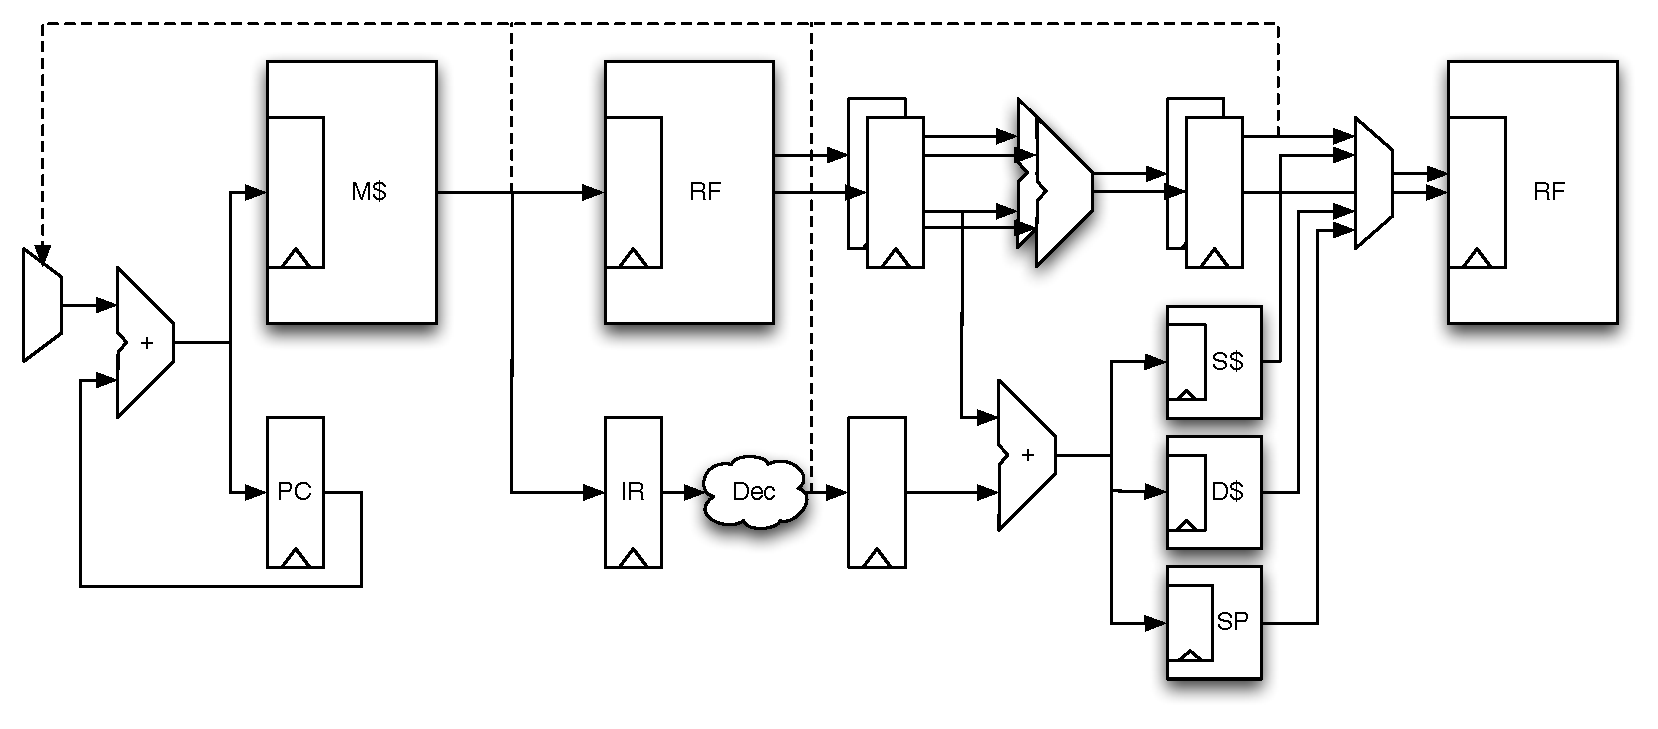
\includegraphics[width=\textwidth]{figures/pipeline}
\end{frame}

\begin{frame}[allowframebreaks]{Instruction Set}
  \begin{itemize}
  \item 3 register ALU instructions
  \item Immediate ALU instructions
    \begin{itemize}
    \item Short and long ALU (2nd issue slot)
    \end{itemize}
  \item Load/store with register + offset
    \begin{itemize}
    \item Word, half word, byte
    \item Aligned access
    \item Typed load/store for different data caches
    \item Split load
    \end{itemize}
    \framebreak
  \item Branch with offset and register indirect
  \item Call/return/branch-with-cache-fill instructions to support method cache
  \item Compare and predicate operation
  \item Stack cache support instructions
  \item Dual issue
    \begin{itemize}
    \item ALU in both pipelines
    \item Load/store and control flow in 1st pipeline      
    \end{itemize}
  \end{itemize}
\end{frame}

\begin{frame}{Method Cache}
  \begin{itemize}
  \item Caches whole functions
  \item Cache misses only on call/return
  \item Everything else is guaranteed hit
  \item Avoids conflicts between data and instruction cache misses
  \item Limited size: split functions
  \end{itemize}
\end{frame}

\begin{frame}{Stack and Data Caches}
  \begin{itemize}
  \item Stack cache
    \begin{itemize}
    \item Stack access behavior regular
    \item Unknown addresses complicate analysis
    \item Split data and stack caches simplify analysis
    \item Reserve/ensure/free inserted by compiler
    \item Spill and fill in hardware
    \end{itemize}
  \item Data cache
    \begin{itemize}
    \item ``Normal'' data cache
    \item Whatever WCET analysis recommends
    \end{itemize}
  \end{itemize}
\end{frame}

\begin{frame}{Simulator}
  \begin{itemize}
  \item Faithful emulation of Patmos
  \item Pipeline model
    \begin{itemize}
    \item Forwarding, stalling, delay slots
    \end{itemize}
  \item Stack, method, and data cache
  \item Intended as design aid
    \begin{itemize}
    \item Compiler development
    \item Runtime statistics
    \item Support execution tracing
    \end{itemize}
  \end{itemize}  
\end{frame}

\begin{frame}{Hardware}
  \begin{itemize}
  \item Complete ISA coverage
  \item Executes normal C programs
  \item Method and data cache
  \item Hardware described in Chisel
    \begin{itemize}
    \item C++-based emulator
    \item FPGA implementation (Verilog)
    \end{itemize}
  \item First multicore versions
  \end{itemize}
\end{frame}

\section{Compilation}

\begin{frame}{Overview}
  \tableofcontents[currentsection]
\end{frame}

\begin{frame}{Compiler}
  \begin{itemize}
  \item Based on LLVM
    \begin{itemize}
    \item Modern open-source compiler
    \item Bitcode as intermediate representation
    \end{itemize}
  \item Linking at bitcode level
    \begin{itemize}
    \item Whole-program optimization
    \item Optimize library code (inlining, \dots)
    \end{itemize}
  \end{itemize}
\end{frame}

\begin{frame}{Special Features}
  \begin{itemize}
  \item Integration of compiler and WCET analysis
  \item Supporting Patmos-specific features
    \begin{itemize}
    \item Example: Function splitting
    \end{itemize}
  \item Single-path code generation
  \item Optimisation based on WCET-feedback
    \begin{itemize}
    \item Example: Cache bypass optimisation
    \end{itemize}
  \end{itemize}
\end{frame}

\begin{frame}{Compilation Flow}
  \begin{columns}
    \begin{column}{.55\textwidth}
      \includegraphics[width=\textwidth]{figures/compiler1}      
    \end{column}
    \begin{column}{.45\textwidth}
      \begin{itemize}
      \item Compile to bitcode
      \item Link bitcode
      \item Optimize
      \item Translate to machine code
      \item Create binary
      \end{itemize}
    \end{column}
  \end{columns}
\end{frame}

\begin{frame}[shrink=30]{Compilation Flow for WCET}
  \begin{columns}
    \begin{column}{.55\textwidth}
      \includegraphics[width=\textwidth]{figures/compiler2}      
    \end{column}
    \begin{column}{.45\textwidth}
      \begin{itemize}
      \item Platin: Portable LLVM Annotation and Timing Toolkit
      \item Export structural and flow information on IR and machine
        code level
      \item PML (Patmos Metainfo Language) file format
      \item Information exchange between compiler and WCET analysis
      \end{itemize}
    \end{column}    
  \end{columns}
\end{frame}

\begin{frame}[allowframebreaks]{Compiler -- WCA Integration}
  \begin{itemize}
  \item Provide information to \emph{enable} WCET analysis
    \begin{itemize}
    \item Structural information
      \begin{itemize}
      \item Branch targets, targets of jump tables
      \end{itemize}
    \item Flow information
      \begin{itemize}
      \item Loop bounds (compiler often knows them!)
      \end{itemize}
    \item Patmos-specific information
      \begin{itemize}
      \item Stack depth for stack cache
      \end{itemize}
    \end{itemize}
    \framebreak
  \item Provide information to \emph{improve} WCET analysis results
    \begin{itemize}
    \item Parametric loop bounds
      \begin{itemize}
      \item Loop bounds that depend on function argument
      \end{itemize}
    \item Targets of memory accesses
      \begin{itemize}
      \item \texttt{instruction ".LBB1\_4"+92 accesses "bit"}
      \end{itemize}
    \end{itemize}
    \framebreak
  \item Import information from WCET analysis
    \begin{itemize}
    \item Basic block execution times and worst-case frequencies
    \item Value analysis results
    \item Worst case execution time      
    \end{itemize}
  \item Used as static profiling information to drive WCET-oriented optimisations
    \begin{itemize}
    \item ``WCET criticalities''
    \end{itemize}
  \end{itemize}
\end{frame}

\begin{frame}{WCET Optimizations}
  \begin{itemize}
  \item Example: Bypass optimisation
    \begin{itemize}
    \item Idea: bypass cache for unpredictable memory accesses
    \item Prevents spoiling the abstract cache state with
      unpredictable cache updates
    \item Exploits Patmos-specific feature: typed loads (and stores)
    \item Uses feedback from WCET Analysis: computed ranges of memory
      addresses
    \end{itemize}
  \end{itemize}
\end{frame}

\begin{frame}{Bypass Optimization}
  \begin{itemize}
  \item Example: 2-way LRU
  \end{itemize}
  \begin{center}
  \includegraphics[width=.85\textwidth]{figures/bypass}    
  \end{center}
\end{frame}

\section{Network-on-Chip}

\begin{frame}{Overview}
  \tableofcontents[currentsection]
\end{frame}

\begin{frame}{Network on Chip}
  \begin{itemize}
  \item Two types of traffic:
    \begin{itemize}
    \item Processor to processor
      \begin{itemize}
      \item DMA driven block transfers SPM $\rightarrow$ SPM (message passing)
      \item Nature: All-to-all
      \end{itemize}
    \item Processor to shared memory (SDRAM)
      \begin{itemize}
      \item Arbitration in NoC \emph{and} in memory controller
      \item Nature: All-towards-one
      \end{itemize}
    \end{itemize}
  \item Globally-asynchronous locally-synchronous (GALS)
    implementation of platform
  \end{itemize}  
\end{frame}

\begin{frame}{NoC Centric View}
  \begin{center}
  \includegraphics[width=.85\textwidth]{figures/noc}    
  \end{center}
\end{frame}

\begin{frame}{Real-Time NoC}
  \begin{itemize}
  \item NoC for real-time systems
  \item Include NoC latency in WCET analysis
    \begin{itemize}
    \item Note: most NoCs are not time-predictable
    \end{itemize}
  \item Statically scheduled arbitration
  \item Time-division multiplexing
    \begin{itemize}
    \item End to end virtual circuits
    \item HW implementation is simple and fast
    \end{itemize}
  \end{itemize}
\end{frame}

\begin{frame}{TDM Schedule}
  \begin{itemize}
  \item Static schedule
    \begin{itemize}
    \item Generated off-line
    \end{itemize}
  \item All-to-all communication
    \begin{itemize}
    \item N $\times$ (N-1) virtual circuits
    \end{itemize}
  \item Has a period
  \item Single word scheduling simplifies schedule generation
  \end{itemize}
\end{frame}

\begin{frame}{Period Bounds}
  \begin{itemize}
  \item A TDM round includes all communication needs
  \item That round is the TDM period
  \item Period determines maximum latency
  \item Minimize schedule period
    \begin{itemize}
    \item We found optimal solutions
      \begin{itemize}
      \item Up to 5x5
      \end{itemize}
    \item Heuristics for larger NoCs
      \begin{itemize}
      \item Nice solution for regular structures
      \end{itemize}
    \end{itemize}
  \end{itemize}  
\end{frame}

\begin{frame}{Argo: the T-CREST NoC}
  \begin{itemize}
  \item TDM-based NoC
  \item Source routing
  \item 3 stage pipelined router
    \begin{itemize}
    \item Synchronous and asynchronous
    \item 3 word packet
    \end{itemize}
  \item Network interface (NI)
    \begin{itemize}
    \item Ticks at TDM clock (mesochronous)
      \begin{itemize}
      \item Drives the asynchronous network
      \end{itemize}
    \item SPM for clock domain crossing    
    \item Time shared DMA machinery
    \end{itemize}
  \end{itemize}  
\end{frame}

\begin{frame}{Argo NI Key Features}
  \begin{itemize}
  \item SPM used for clock domain crossing
    \begin{itemize}
    \item One DMA needed per connection
    \item Only one active at any time due to TDM
    \end{itemize}
  \item Enables efficient table-based implementation of DMA controllers
  \item End-to-end (i.e., SPM-to-SPM) data transfer
    \begin{itemize}
    \item Avoids buffering and flow control
    \end{itemize}
  \end{itemize}  
\end{frame}

\begin{frame}{Discussion}
  \begin{itemize}
  \item TDM wastes bandwidth
  \item All-to-all schedule wastes even more!
    \begin{itemize}
    \item Does it matter?
    \end{itemize}
  \item There is plenty of bandwidth on-chip
    \begin{itemize}
    \item Wires are cheap
    \item 1024 bit wide busses in an FPGA possible
    \end{itemize}
  \item TDM all-to-all routers are cheap
  \item Bandwidth relative to cost matters
  \end{itemize}
\end{frame}

\section{Memory Access}

\begin{frame}{Overview}
  \tableofcontents[currentsection]
\end{frame}

\begin{frame}{Memory Tree}
  \begin{itemize}
  \item Access to memory is all-towards-one
  \item Processors are leaves, memory is root
  \item Hierarchy of simple arbitration elements (multiplexers/``routers'')
  \end{itemize}
  \begin{center}
  \includegraphics[width=.5\textwidth]{figures/memtree}    
  \end{center}
\end{frame}

\begin{frame}{Memory Controller}
  \begin{itemize}
  \item DRAM access complex
    \begin{itemize}
    \item Row activation, precharging, \dots
    \end{itemize}
  \item Standard controllers do heavy reordering for performance
    \begin{itemize}
    \item Poor predictability
    \end{itemize}
  \item Good: Patterns with guaranteed timing
  \item Better: \emph{Controlled} dynamic reordering
    \begin{itemize}
    \item Same worst-case behavior as patterns
    \item Better average-case performance
    \end{itemize}
  \end{itemize}
\end{frame}

\section{Summary}

\begin{frame}{Overview}
  \tableofcontents[currentsection]
\end{frame}

\begin{frame}{Summary}
  \begin{itemize}
  \item New computer architecture for real-time systems
  \item WCET analyzability is of primary importance
  \item T-CREST is a platform
    \begin{itemize}
    \item Processor, NoC, memory controller, compiler, WCET analysis
    \end{itemize}
  \item Technology is mostly open source
    \begin{itemize}
    \item Usage and collaboration are VERY welcome
    \end{itemize}
  \end{itemize}
\end{frame}

\begin{frame}{More Information}
  \begin{itemize}
  \item T-CREST
    \begin{itemize}
    \item \url{http://t-crest.org}
    \item Most deliverables are public
    \end{itemize}
  \item Patmos web site
    \begin{itemize}
    \item \url{http://patmos.compute.dtu.dk}
    \end{itemize}
  \item Development
    \begin{itemize}
    \item Most artifacts are open source
    \item GitHub: \url{http://github.com/t-crest}
    \end{itemize}
  \end{itemize}
\end{frame}

\section{Demo}

\begin{frame}{Overview}
  \tableofcontents[currentsection]
\end{frame}

\begin{frame}{Uniprocessor Demo}
  \begin{itemize}
  \item Single core
    \begin{itemize}
    \item ROM with boot loader
    \end{itemize}
  \item Application written in C
    \begin{itemize}
    \item Mandelbrot generator
    \item Compiled with \texttt{patmos-clang}
    \end{itemize}
  \item Communication with processor via serial line
    \begin{itemize}
    \item Image display on laptop
    \end{itemize}
  \end{itemize}
\end{frame}

\begin{frame}{<Demo>}
  \begin{itemize}
  \item Compilation
  \item FPGA configuration
  \item Download
  \item Execution
  \end{itemize}
\end{frame}

\begin{frame}{Multiprocessor Demo}
  \begin{itemize}
  \item Nine cores, connected through on-chip network
    \begin{itemize}
    \item One master, eight slaves
    \item Master downloads application
    \end{itemize}
  \item Application written in C
    \begin{itemize}
    \item Mandelbrot generator
    \item Compiled with \texttt{patmos-clang}
    \end{itemize}
  \item Communication with processor via serial line
    \begin{itemize}
    \item Image display on laptop
    \item Use \texttt{ed} to update image step by step
    \end{itemize}
  \end{itemize}
\end{frame}

\end{document}
